\documentclass[tikz, margin=3mm]{standalone}
\usepackage{tikz}
\usepackage{amsmath}
\usepackage{comment}
\usetikzlibrary{shapes.geometric, arrows, positioning}
\tikzstyle{arrow} = [thick,->,>=stealth]

% flow chart of simulation (zoomed out view)
% uses relative positioning

% Terminal
\tikzstyle{terminal} = [rectangle, rounded corners, minimum width=3cm, minimum height=1cm,text centered, text width=3cm, draw=black]

% Process
\tikzstyle{process} = [rectangle, minimum width=3cm, minimum height=1cm, text centered,text width=4cm, draw=black]

% Decision
\tikzstyle{decision} = [diamond, aspect=1.8, minimum width=2cm, minimum height=1cm, text centered, text width=2cm, draw=black]

% Subprocess
\newcommand\ppbb{path picture bounding box}
\tikzset{
	subprocess/.style = {rectangle, draw=black, 
		minimum width=4.3cm, minimum height=1cm, inner xsep=3mm,
		text width =\pgfkeysvalueof{/pgf/minimum width}-2*\pgfkeysvalueof{/pgf/inner xsep},
		align=flush center,
		path picture={\draw 
			([xshift =2mm] \ppbb.north west) -- ([xshift= 2mm] \ppbb.south west)
			([xshift=-2mm] \ppbb.north east) -- ([xshift=-2mm] \ppbb.south east);
		},% end of path picture
	}
}

\tikzstyle{note} = [fill, ellipse,fill=gray!20, node distance=4cm, minimum height=1em, text width=3cm, text centered]

\begin{document}
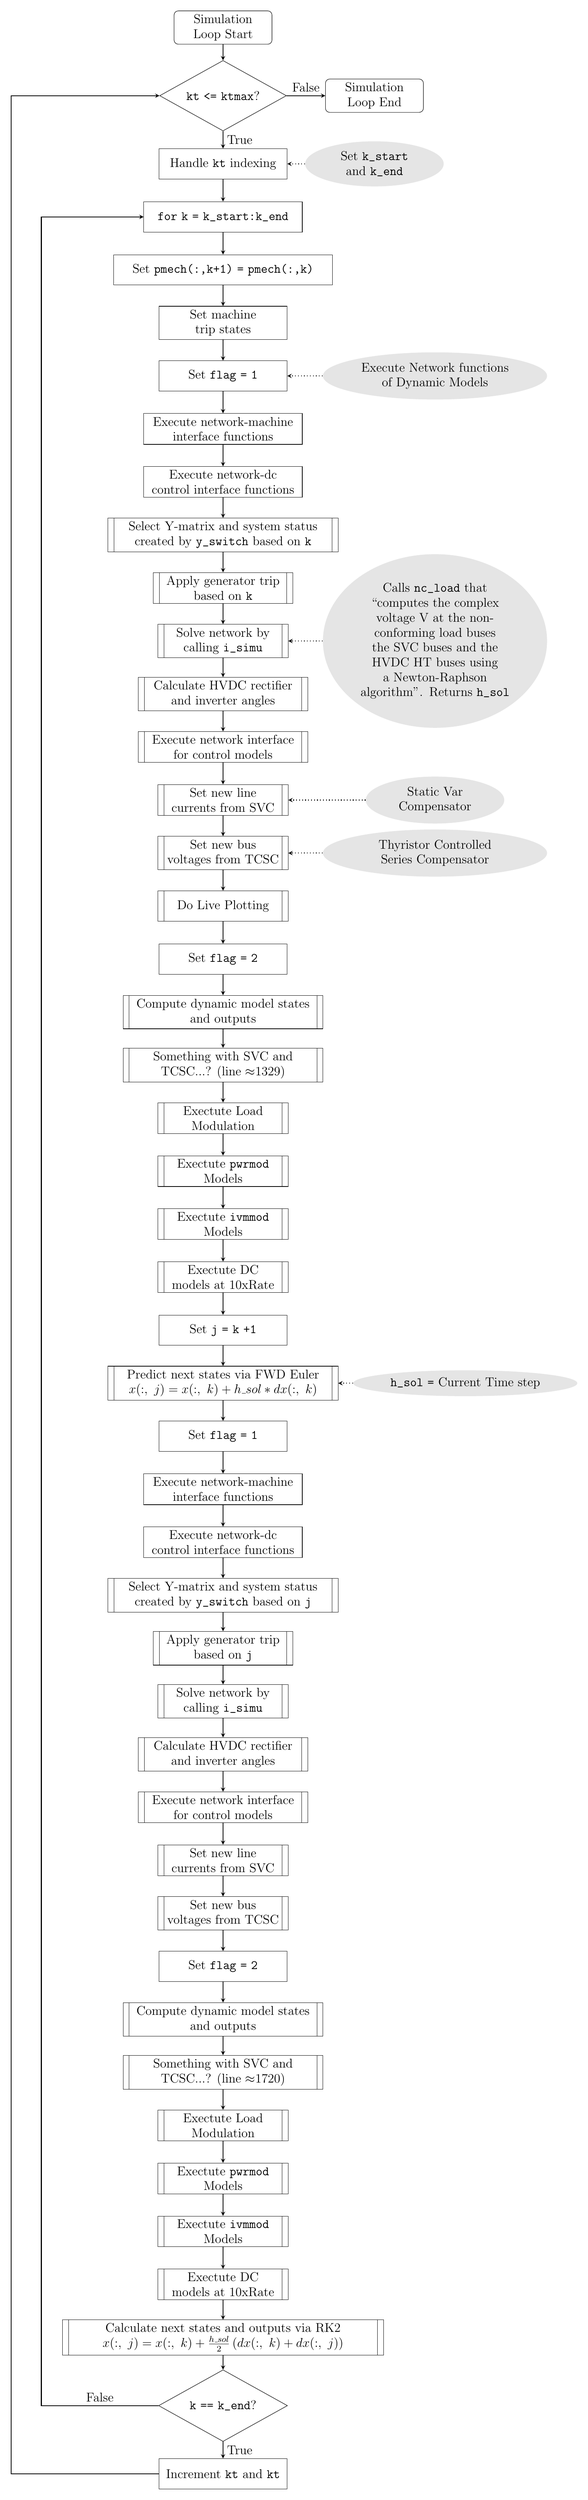
\begin{tikzpicture}[node distance=1.75cm, font=\large] 
%================================================================================================
% Placement of flowcart nodes
\node (simLoopStart) [terminal] {Simulation Loop Start};
\node (whileKT) [decision, below of=simLoopStart, yshift=-.5cm, text width=3cm] {\verb|kt <= ktmax|?};
\node (KTindex) [process, below of = whileKT, yshift=-.5cm] {Handle \verb|kt| indexing};
\node (simLoopEnd) [terminal, right of = whileKT, node distance = 5 cm] {Simulation Loop End};
\node (forKlength) [process, below of = KTindex, text width = 5cm] {\verb|for k = k_start:k_end|};

\node (setPmech) [process, below of = forKlength, text width = 7cm] {Set \verb|pmech(:,k+1) = pmech(:,k)|};
\node (tripGen1) [process, below of = setPmech] {Set machine trip states};
\node (setFlagONE1) [process, below of = tripGen1] {Set \verb|flag = 1|};
\node (machineInterface1) [process, below of = setFlagONE1, text width = 5cm] {Execute network-machine interface functions};

\node (dcCTRLS1) [process, below of = machineInterface1, text width = 5cm] {Execute network-dc control interface functions};
\node (selectSYS1) [subprocess, below of = dcCTRLS1, text width = 7cm] {Select Y-matrix and system status created by \verb|y_switch| based on \verb|k|};
\node (applyGenTrip) [subprocess, below of = selectSYS1, text width = 4cm] {Apply generator trip based on \verb|k|};
\node (solveNetwork1) [subprocess, below of = applyGenTrip] {Solve network by calling \verb|i_simu|};
%line 1212

\node (HVDC1) [subprocess, below of = solveNetwork1, text width = 5 cm] {Calculate HVDC rectifier and inverter angles};
\node (ctrlNetwork1) [subprocess, below of = HVDC1, text width = 5 cm] {Execute network interface for control models};
\node (Isvc1) [subprocess, below of = ctrlNetwork1] {Set new line currents from SVC};
\node (Vtcsc) [subprocess, below of = Isvc1] {Set new bus voltages from TCSC};

\node (LivePlot) [subprocess, below of = Vtcsc] {Do Live Plotting};
\node (setFlagTWO1) [process, below of = LivePlot] {Set \verb|flag = 2|};
\node (dynamics1) [subprocess, below of = setFlagTWO1, text width = 6 cm] {Compute dynamic model states and outputs};
\node (mystery1) [subprocess, below of = dynamics1, text width = 6 cm] {Something with SVC and TCSC...? (line $\approx$1329)};


\node (lmod1) [subprocess, below of = mystery1] {Exectute Load Modulation};
\node (pwrmod1) [subprocess, below of = lmod1] {Exectute \verb|pwrmod| Models};
\node (ivmmod1) [subprocess, below of = pwrmod1] {Exectute \verb|ivmmod| Models};
\node (HVDCint1) [subprocess, below of = ivmmod1] {Exectute DC models at 10xRate};

\node (setJ) [process, below of = HVDCint1] {Set \verb|j = k +1|};
\node (fwdEuler1) [subprocess, below of = setJ, text width = 7cm] {Predict next states via FWD Euler $x(:,\ j) = x(:,\ k)+ h\_sol*dx(:,\ k)$};

%--------------------------------------------------------------------------------------------------
% begining of next solution (i.e. 'corrector')

\node (setFlagONE2) [process, below of = fwdEuler1] {Set \verb|flag = 1|};
\node (machineInterface2) [process, below of = setFlagONE2, text width = 5cm] {Execute network-machine interface functions};

\node (dcCTRLS2) [process, below of = machineInterface2, text width = 5cm] {Execute network-dc control interface functions};
\node (selectSYS2) [subprocess, below of = dcCTRLS2, text width = 7cm] {Select Y-matrix and system status created by \verb|y_switch| based on \verb|j|};
\node (applyGenTrip2) [subprocess, below of = selectSYS2, text width = 4cm] {Apply generator trip based on \verb|j|};
\node (solveNetwork2) [subprocess, below of = applyGenTrip2] {Solve network by calling \verb|i_simu|};

\node (HVDC2) [subprocess, below of = solveNetwork2, text width = 5 cm] {Calculate HVDC rectifier and inverter angles};
\node (ctrlNetwork2) [subprocess, below of = HVDC2, text width = 5 cm] {Execute network interface for control models};
\node (Isvc2) [subprocess, below of = ctrlNetwork2] {Set new line currents from SVC};
\node (Vtcsc2) [subprocess, below of = Isvc2] {Set new bus voltages from TCSC};

\node (setFlagTWO2) [process, below of = Vtcsc2] {Set \verb|flag = 2|};
\node (dynamics2) [subprocess, below of = setFlagTWO2, text width = 6 cm] {Compute dynamic model states and outputs};
\node (mystery2) [subprocess, below of = dynamics2, text width = 6 cm] {Something with SVC and TCSC...? (line $\approx$1720)};

\node (lmod2) [subprocess, below of = mystery2] {Exectute Load Modulation};
\node (pwrmod2) [subprocess, below of = lmod2] {Exectute \verb|pwrmod| Models};
\node (ivmmod2) [subprocess, below of = pwrmod2] {Exectute \verb|ivmmod| Models};
\node (HVDCint2) [subprocess, below of = ivmmod2] {Exectute DC models at 10xRate};

\node (RK2) [subprocess, below of = HVDCint2, text width = 10cm] {Calculate next states and outputs via RK2 $x(:,\ j) = x(:,\ k)+ \frac{ h\_sol}{2} \left(dx(:,\ k) + dx(:,\ j) \right)$};
\node (forOver) [decision, below of=RK2, yshift=-.5cm, text width=3cm] {\verb|k == k_end|?};
\node (counterInc) [process, below of = forOver, yshift=-.5cm] {Increment \verb|kt| and \verb|kt|};

%================================================================================================
% Drawing of Lines of main chart
\draw [arrow] (simLoopStart) -- (whileKT);
\draw [arrow] (KTindex) -- (forKlength);
\draw [arrow] (forKlength) -- (setPmech);

\draw [arrow] (setPmech) -- (tripGen1);
\draw [arrow] (tripGen1) -- (setFlagONE1);
\draw [arrow] (setFlagONE1) -- (machineInterface1);
\draw [arrow] (machineInterface1) -- (dcCTRLS1);

\draw [arrow] (dcCTRLS1) -- (selectSYS1);
\draw [arrow] (selectSYS1) -- (applyGenTrip);
\draw [arrow] (applyGenTrip) -- (solveNetwork1);
\draw [arrow] (solveNetwork1) -- (HVDC1);

\draw [arrow] (HVDC1) -- (ctrlNetwork1);
\draw [arrow] (ctrlNetwork1) -- (Isvc1);
\draw [arrow] (Isvc1) -- (Vtcsc);
\draw [arrow] (Vtcsc) -- (LivePlot);

\draw [arrow] (LivePlot) -- (setFlagTWO1);
\draw [arrow] (setFlagTWO1) -- (dynamics1);
\draw [arrow] (dynamics1) -- (mystery1);
\draw [arrow] (mystery1) -- (lmod1);

\draw [arrow] (lmod1) -- (pwrmod1);
\draw [arrow] (pwrmod1) -- (ivmmod1);
\draw [arrow] (ivmmod1) -- (HVDCint1);
\draw [arrow] (HVDCint1) -- (setJ);

\draw [arrow] (setJ) -- (fwdEuler1);
% begining of next solution (i.e. 'corrector')
\draw [arrow] (fwdEuler1) -- (setFlagONE2);
\draw [arrow] (setFlagONE2) -- (machineInterface2);
\draw [arrow] (machineInterface2) -- (dcCTRLS2);

\draw [arrow] (dcCTRLS2) -- (selectSYS2);
\draw [arrow] (selectSYS2) -- (applyGenTrip2);
\draw [arrow] (applyGenTrip2) -- (solveNetwork2);
\draw [arrow] (solveNetwork2) -- (HVDC2);

\draw [arrow] (HVDC2) -- (ctrlNetwork2);
\draw [arrow] (ctrlNetwork2) -- (Isvc2);
\draw [arrow] (Isvc2) -- (Vtcsc2);
\draw [arrow] (Vtcsc2) -- (setFlagTWO2);

\draw [arrow] (setFlagTWO2) -- (dynamics2);
\draw [arrow] (dynamics2) -- (mystery2);
\draw [arrow] (mystery2) -- (lmod2);

\draw [arrow] (lmod2) -- (pwrmod2);
\draw [arrow] (pwrmod2) -- (ivmmod2);
\draw [arrow] (ivmmod2) -- (HVDCint2);
\draw [arrow] (HVDCint2) -- (RK2);

\draw [arrow] (RK2) -- (forOver);
\draw [arrow] (counterInc) --  +(-7,0) |- (whileKT);

%================================================================================================
% Draw Decision Lines
\draw [arrow] (whileKT) --  node[anchor=west] {True} (KTindex);
\draw [arrow] (whileKT) --  node[anchor=south] {False} (simLoopEnd);

\draw [arrow] (forOver) --  node[anchor=west] {True} (counterInc);
\draw [arrow] (forOver) -- node[anchor=south, midway] {False} +(-6,0) |- (forKlength);
%================================================================================================
%% Note nodes AND edges
\node [note, right of=KTindex, node distance =5cm](note1){Set \verb|k_start| and \verb|k_end|};
\draw [arrow,dotted] (note1) -- (KTindex);

\node [note, right of=setFlagONE1, node distance =7cm, text width = 5cm](note2){Execute Network functions of Dynamic Models};
\draw [arrow,dotted] (note2) -- (setFlagONE1);

\node [note, right of=solveNetwork1, node distance =7cm, text width = 5cm](note3){Calls \verb|nc_load| that ``computes the complex voltage V at the non-conforming load buses
the SVC buses and the HVDC HT buses using a Newton-Raphson algorithm". Returns \verb|h_sol|};
\draw [arrow,dotted] (note3) -- (solveNetwork1);

\node [note, right of=Isvc1, node distance =7cm, ](note4){Static Var Compensator};
\draw [arrow,dotted] (note4) -- (Isvc1);

\node [note, right of=Vtcsc, node distance =7cm, text width = 5 cm ](note5){Thyristor Controlled Series Compensator};
\draw [arrow,dotted] (note5) -- (Vtcsc);

\node [note, right of=fwdEuler1, node distance =8cm, text width = 5 cm ](note5){\verb|h_sol = |Current Time step}; % $\approx$Line 1468
\draw [arrow,dotted] (note5) -- (fwdEuler1);
\end{tikzpicture}

\begin{comment}
% Basic flowchart example
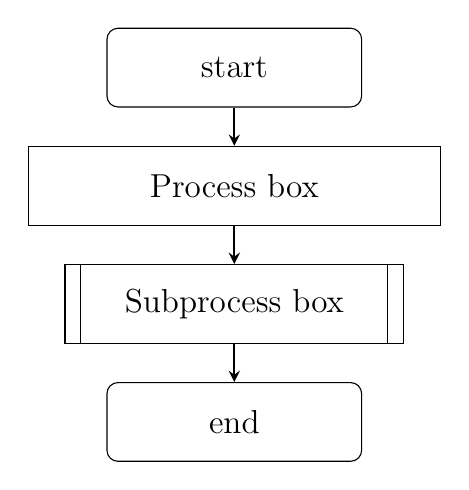
\begin{tikzpicture}[node distance=1.5cm, font=\large] 
% Placement of flowcart nodes
\node (term1) [terminal] {start};
\node (proc1) [process, below of = term1,text width=5cm] {Process box};% optional text width
\node (sproc1) [subprocess, below of = proc1] {Subprocess box};
\node (term2) [terminal, below of = sproc1] {end};

% Drawing of Lines
\draw [arrow] (term1) -- (proc1);
\draw [arrow] (proc1) -- (sproc1);
\draw [arrow] (sproc1) -- (term2);

\end{tikzpicture}


% Taken from PSLTDSim flowchart - here as a reference
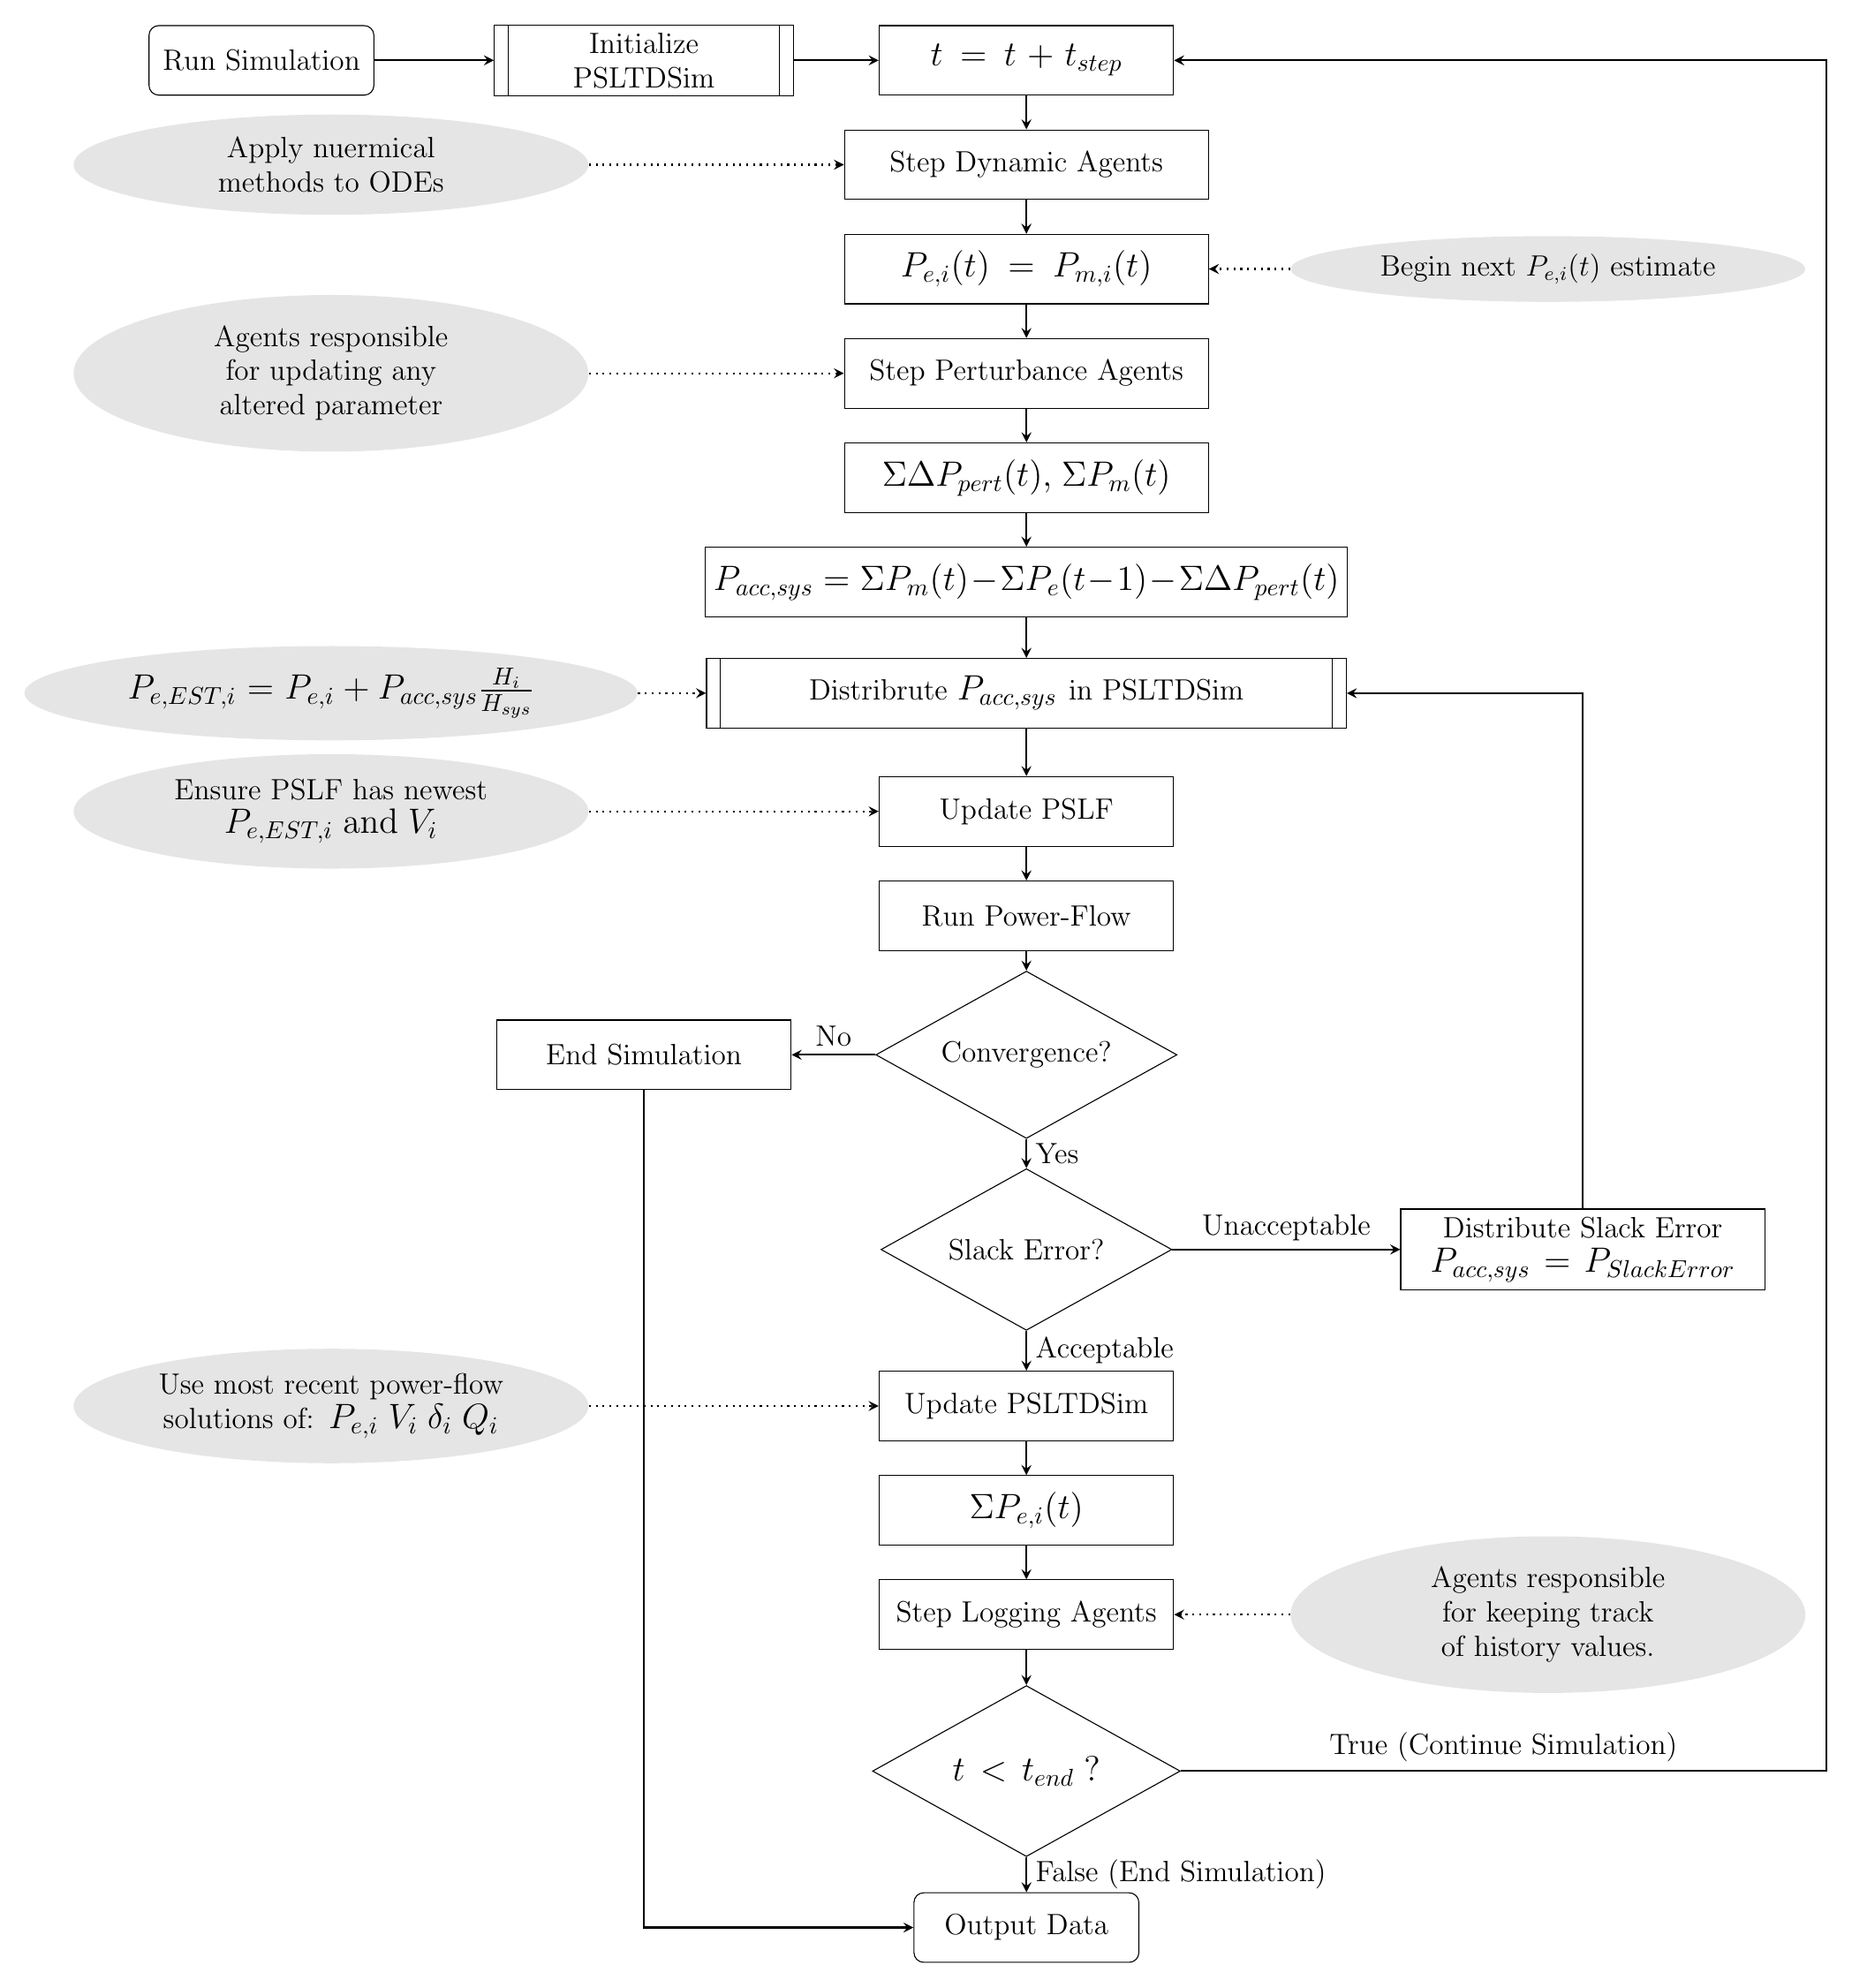
\begin{tikzpicture}[node distance=1.5cm, font=\large] 
% Placement of nodes
\node (start) [terminal] {Run Simulation};
\node (init) [subprocess, right of=start,xshift=4cm] {Initialize PSLTDSim};
\node (tStep) [process, right of=init,xshift=4cm] {\Large$t = t+t_{step}$};
\node (dyStep) [process, below of=tStep,text width=5cm] {Step Dynamic Agents};
\node (PeEst) [process, below of=dyStep,text width=5cm] {\Large$P_{e,i}(t) = P_{m,i}(t)$};
\node (stepPert) [process, below of=PeEst, text width=5cm] {Step Perturbance Agents};
\node (sumPertPm) [process, below of=stepPert, text width=5cm] {\Large$\Sigma\Delta P_{pert}(t)$, $\Sigma P_{m}(t)$};
\node (calcPacc)[process, below of=sumPertPm,  text width=9cm] {\Large$P_{acc, sys} = \Sigma P_m(t)-\Sigma P_e(t-1)- \Sigma \Delta P_{pert}(t)$};
\node (distPe) [subprocess, below of=calcPacc,yshift=-.1cm, text width=8.6cm] { Distribrute \Large$P_{acc, sys}$ \large in PSLTDSim};
\node (updatePSLF) [process, below of=distPe, yshift=-.2cm] {Update PSLF};
\node (runPF) [process, below of=updatePSLF,text width=4cm] {Run Power-Flow};

%Convergence nodes
\node (pfConv) [decision, below of=runPF, yshift=-.5cm, text width=3cm] {Convergence?};
\node (pfFail) [process, left of=pfConv, xshift=-4cm] {End Simulation};
%Slack error nodes
\node (slackErr) [decision, below of=pfConv, yshift=-1.3cm, text width=3cm] {Slack Error?};
\node (slackTol) [process, right of=slackErr, xshift=6.5cm, text width = 5cm] {Distribute Slack Error \\ \Large$P_{acc, sys} = P_{SlackError}$};

\node (updateLTD) [process, below of=slackErr,yshift=-0.75cm] {Update PSLTDSim};
\node (sumPe) [process,below of=updateLTD] {\Large$\Sigma P_{e,i}(t)$};
\node (log) [process, below of=sumPe, text width = 4cm] {Step Logging Agents};
\node (loop) [decision, below of=log, yshift=-.75cm, text width=3cm] {\Large$t<t_{end}$ ?};
\node (dataOut) [terminal, below of=loop, yshift=-.75cm] {Output Data};

%% Note nodes AND edges
\node [note, left of=updatePSLF, node distance =10cm,text width=5cm](note1){Ensure PSLF has newest \Large $P_{e,EST,i}$ and $V_{i}$};
\draw [arrow,dotted] (note1) -- (updatePSLF);

\node [note, left of=updateLTD, node distance =10cm, text width=5cm](note2){Use most recent power-flow solutions of: \Large $P_{e,i}\  V_i\  \delta_i \ Q_i$};
\draw [arrow,dotted] (note2) -- (updateLTD);

\node [note, left of=stepPert, node distance =10cm, text width=5cm](note3){Agents responsible for updating any altered parameter};
\draw [arrow,dotted] (note3) -- (stepPert);

\node [note, left of=dyStep, node distance =10cm, text width=5cm](note4){Apply nuermical methods to ODEs};
\draw [arrow,dotted] (note4) -- (dyStep);

\node [note, right of=PeEst, node distance =7.5cm, text width=5cm](note5){Begin next $P_{e,i}(t)$ estimate };
\draw [arrow,dotted] (note5) -- (PeEst);

\node [note, right of=log, node distance =7.5cm, text width=5cm](note6){Agents responsible for keeping track of history values.};
\draw [arrow,dotted] (note6) -- (log);

\node [note, left of=distPe, node distance =10cm, text width=6cm](note7){\Large$P_{e,EST,i}= P_{e,i} +P_{acc, sys}\frac{H_i}{H_{sys}}$};
\draw [arrow,dotted] (note7) -- (distPe);

% Placement of edges
\draw [arrow] (start) -- (init);
\draw [arrow] (init) -- (tStep);
\draw [arrow] (tStep) -- (dyStep);
\draw [arrow] (dyStep) -- (PeEst);
\draw [arrow] (PeEst) -- (stepPert);
\draw [arrow] (stepPert) -- (sumPertPm);
\draw [arrow] (sumPertPm) -- (calcPacc);
\draw [arrow] (calcPacc) -- (distPe);
\draw [arrow] (distPe) -- (updatePSLF);
\draw [arrow] (updatePSLF) -- (runPF);
\draw [arrow] (runPF) -- (pfConv);

% pf convergence bad
\draw [arrow] (pfConv) --  node[anchor=south] {No} (pfFail);
\draw [arrow] (pfFail) |-  (dataOut);
% pf convergence ok
\draw [arrow] (pfConv) --  node[anchor=west] {Yes} (slackErr);

% slack tolerance bad
\draw [arrow] (slackErr) --  node[anchor=south] {Unacceptable} (slackTol);
\draw [arrow] (slackTol) |- (distPe);
% slack tolerance ok
\draw [arrow] (slackErr) --  node[anchor=west] {Acceptable} (updateLTD);

\draw [arrow] (updateLTD) --(sumPe);
\draw [arrow] (sumPe) --(log);
\draw [arrow] (log) --(loop);

%loop again
\draw [arrow] (loop) -- node[anchor=south, midway] {True (Continue Simulation)} +(11.5,0) |- (tStep);
% end simulation
\draw [arrow] (loop) -- node[anchor=west] {False (End Simulation)} (dataOut);
\end{tikzpicture}
\end{comment}
\end{document}
